\chapter{Результаты}
Для демонстрации работы критерия предоставленны 10 полей ввода. Оценка производятся для целых чисел от 0 до 9. Примеры работы программы приведены на рисунках \ref{p1}--\ref{p3}.

\begin{figure}[h]
	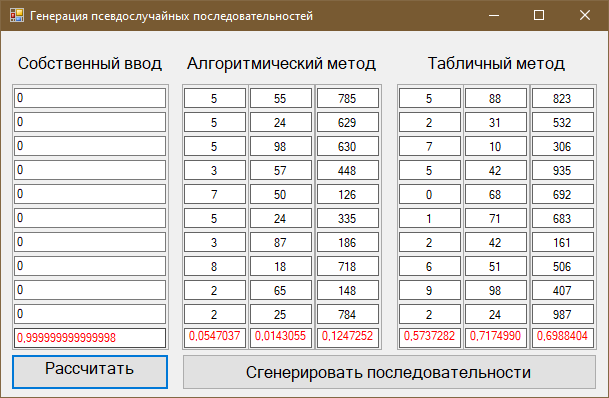
\includegraphics[width=1\linewidth]{inc/img/1.png}
	\caption{Последовательность из одинаковых чисел}
	\label{p1}
\end{figure}

\begin{figure}[h]
	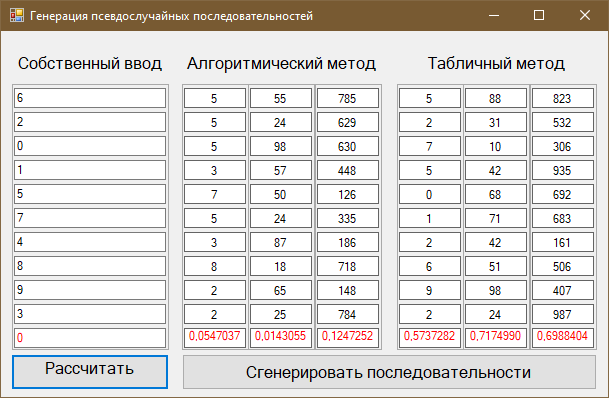
\includegraphics[width=1\linewidth]{inc/img/2.png}
	\caption{Последовательность из чисел от 0 до 9}
	\label{p2}
\end{figure}

\begin{figure}[h]
	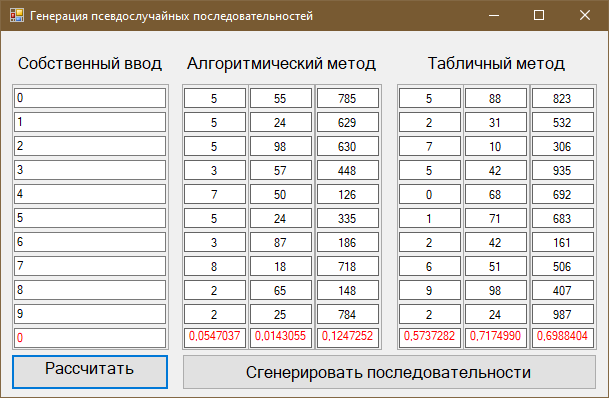
\includegraphics[width=1\linewidth]{inc/img/4.png}
	\caption{Возрастающая последовательность}
	\label{p4}
\end{figure}

\begin{figure}[h]
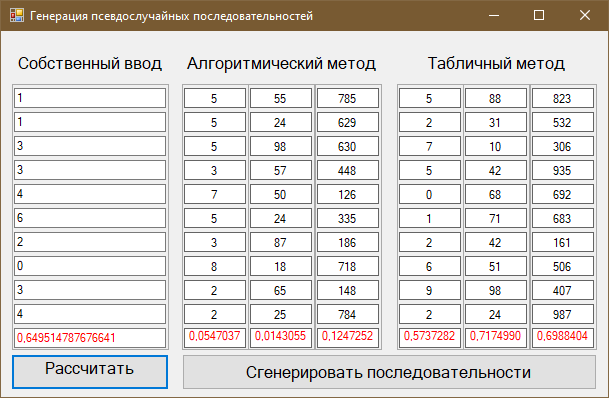
\includegraphics[width=1\linewidth]{inc/img/3.png}
\caption{Введена случайная последовательность}
\label{p3}
\end{figure}
